\documentclass[aspectratio=169,12pt,handout]{beamer}
\usepackage{pgfpages}
\pgfpagesuselayout{resize to}[letterpaper,landscape,border shrink=5mm]
\usetheme{Madrid}
\usecolortheme{default}
\usepackage{graphicx}
\usepackage{booktabs}
\usepackage{amsmath}

\definecolor{binggreen}{RGB}{0,100,0}
\setbeamercolor{structure}{fg=binggreen}
\setbeamercolor{title}{fg=white,bg=binggreen}
\setbeamercolor{frametitle}{fg=white,bg=binggreen}

\setbeamertemplate{navigation symbols}{}
\setbeamertemplate{footline}{%
  \vspace*{4mm}\hfill\insertframenumber/\inserttotalframenumber\hspace{2mm}%
}

\hypersetup{pdfpagelayout=SinglePage}

\title{clusterOne: Pearson vs sMAPE}
\subtitle{A Spotlight \;|\; Side-Deck for Week of April 30}
\author{}
\institute{Binghamton University}
\date{April 2026}

\begin{document}

% ------------------------------------------------------------------
\begin{frame}
\titlepage
\end{frame}

% ------------------------------------------------------------------
\begin{frame}{Why This Question}
\small
\begin{itemize}
  \item Main deck picked \textbf{Pearson} for clusterOne (rawMAE failed shape; fall back to principled scale-invariant shape metric).
  \item But sMAPE also passes the dual gate cleanly on clusterOne and looks slightly tighter to the pattern in the mean-shift view.
  \item Both score \textbf{shape $= 1.00$} (every top-20 gene has $r > 0.9$ vs pattern). Both pass the magnitude gate too. Need a tiebreaker.
  \item This deck: visual + numerical comparison so the pick is defended, not assumed.
\end{itemize}
\vspace{0.6em}
\textcolor{binggreen}{\textbf{Verdict (preview):}} Pearson, but for sharper reasons than the main deck stated.
\end{frame}

% ------------------------------------------------------------------
\begin{frame}{The 3-View Comparison}
\centering
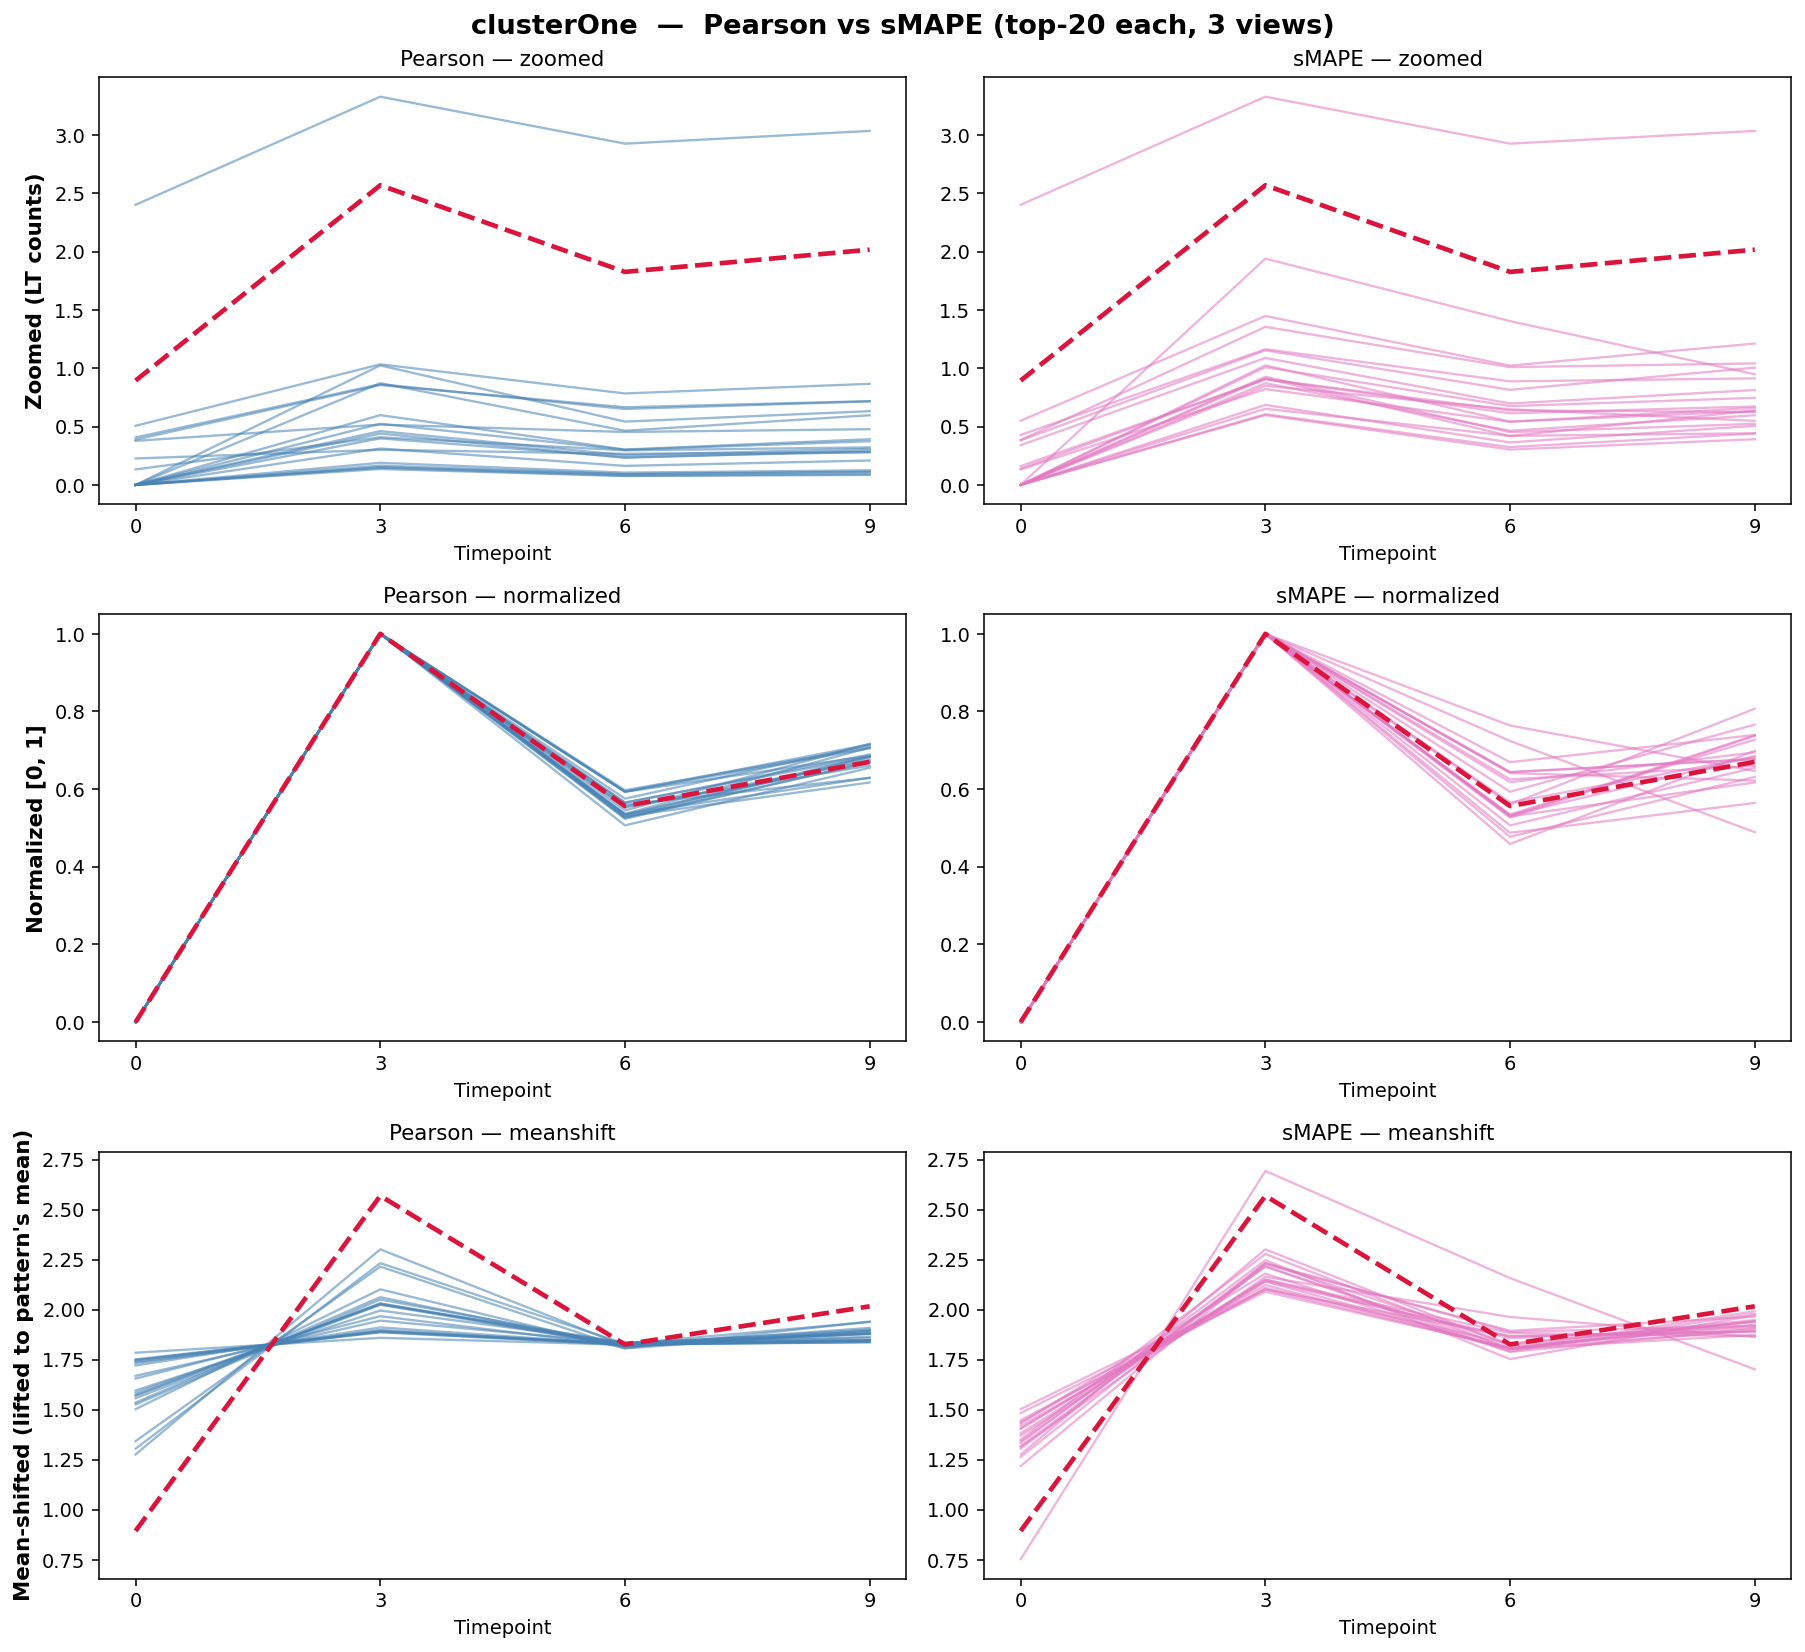
\includegraphics[height=0.85\textheight]{plots/pearson_vs_smape_3views.png}
\end{frame}

% ------------------------------------------------------------------
\begin{frame}{What the Three Views Say}
\small
\begin{itemize}
  \item \textbf{Zoomed:} Pearson genes sit at LT $\sim$ 0--1; sMAPE genes at LT $\sim$ 1--2. sMAPE is visibly closer to the pattern's actual range (0.85--2.55).
  \item \textbf{Normalized:} Pearson shows a tight overlay on the pattern's shape. sMAPE shows visible fanning, especially after $t{=}3$.
  \item \textbf{Mean-shifted:} sMAPE traces the up-down-up spike better; Pearson genes look flatter around the pattern's mean.
\end{itemize}
\vspace{0.4em}
\textcolor{binggreen}{\textbf{So which view do we trust?}} Different views answer different questions. The next two slides ground each in a number so it's not eyeballing.
\end{frame}

% ------------------------------------------------------------------
\begin{frame}{Number 1 --- Amplitude (Why sMAPE Wins Mean-Shift)}
\small
Mean dynamic range (max $-$ min) of each method's top-20 on clusterOne:
\begin{center}
\begin{tabular}{lc}
\toprule
\textbf{Method} & \textbf{Mean LT range} \\
\midrule
Pearson & 0.41 \\
\textbf{sMAPE}  & \textbf{0.87} \;($\sim$2$\times$ Pearson) \\
\midrule
\textit{Pattern itself} & \textit{1.68} \\
\bottomrule
\end{tabular}
\end{center}
\vspace{0.6em}
sMAPE's picks are at \textbf{52\% of the pattern's amplitude}; Pearson's are at \textbf{25\%}.
\vspace{0.4em}
$\Rightarrow$ The mean-shift advantage is \textbf{real}, not an artifact. sMAPE picks higher-amplitude shape-correct genes that more closely trace the pattern's spike when shifted to the same mean.
\end{frame}

% ------------------------------------------------------------------
\begin{frame}{Number 2 --- Shape Consistency (Why Pearson Wins Normalized)}
\centering
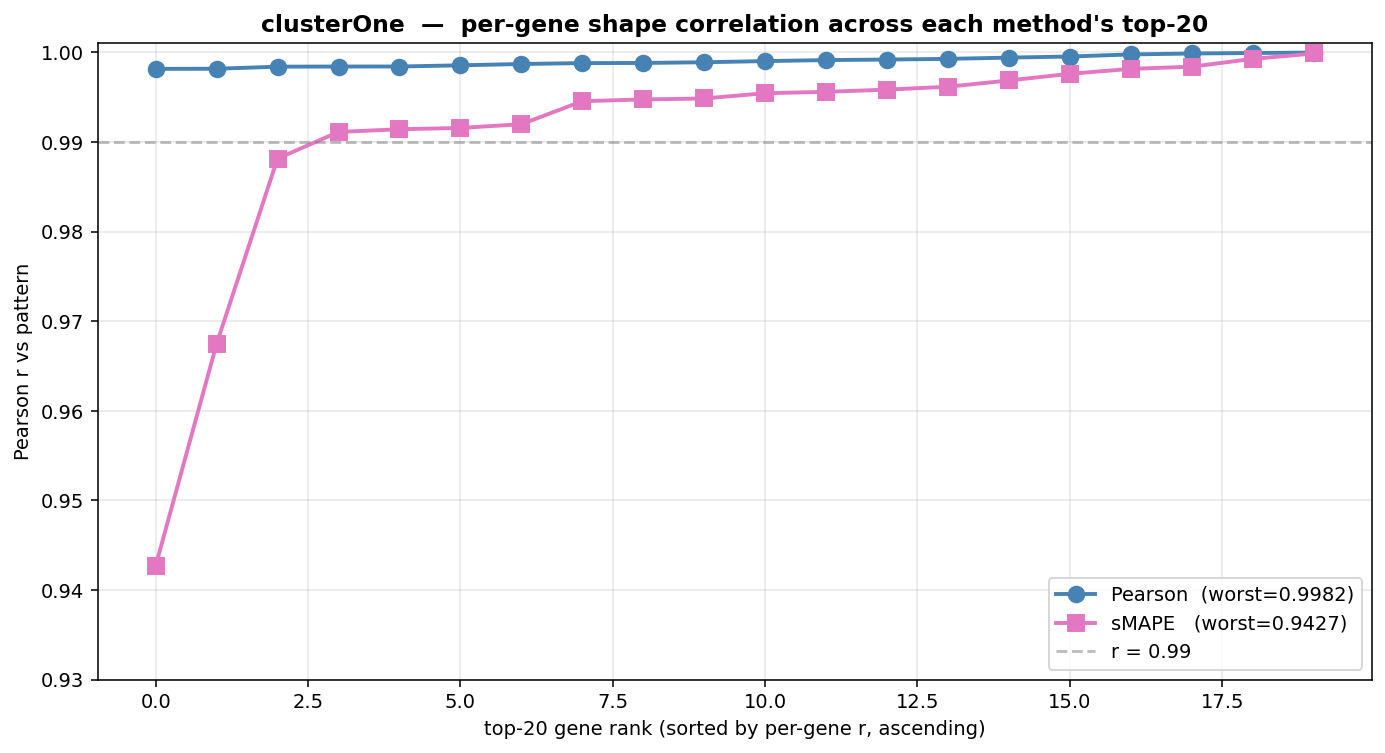
\includegraphics[width=\textwidth]{plots/pearson_vs_smape_r_dist.png}
\end{frame}

% ------------------------------------------------------------------
\begin{frame}{The Per-Gene r Distribution Tells the Whole Story}
\small
\begin{center}
\begin{tabular}{lcccc}
\toprule
\textbf{Method} & \textbf{Worst $r$} & \textbf{Median $r$} & \textbf{$\#\,r > 0.99$} & \textbf{$\#\,r > 0.998$} \\
\midrule
\textbf{Pearson} & \textbf{0.998} & 0.999 & \textbf{20 / 20} & \textbf{20 / 20} \\
sMAPE   & 0.943 & 0.995 & 17 / 20 & 0 / 20 \\
\bottomrule
\end{tabular}
\end{center}
\vspace{0.5em}
\begin{itemize}
  \item \textbf{Pearson}: every one of the 20 picks has $r \geq 0.998$. Essentially perfect shape correlation, top to bottom.
  \item \textbf{sMAPE}: median is comparable, but the bottom 3 of 20 fall below $r = 0.99$, with the worst at $0.94$. Some shape variance is being absorbed.
\end{itemize}
\vspace{0.4em}
\textcolor{binggreen}{\textbf{So the trade is sharp:}} sMAPE buys $\sim$2$\times$ amplitude proximity by accepting noticeable shape variance on the bottom of its top-20. Pearson keeps shape extremely tight at the cost of amplitude.
\end{frame}

% ------------------------------------------------------------------
\begin{frame}{The Verdict}
\small
The trade-off:
\begin{center}
\begin{tabular}{lcc}
\toprule
& \textbf{sMAPE buys} & \textbf{Pearson buys} \\
\midrule
Amplitude proximity & \textbf{52\% of pattern's range} & 25\% \\
Worst-case shape    & 0.94 & \textbf{0.998} \\
Empirical consensus & 4 / 20 with Pearson & --- (set the consensus) \\
\bottomrule
\end{tabular}
\end{center}

\vspace{0.6em}
\textbf{The prof ruled shape $>$ magnitude.} Under that priority:
\begin{itemize}\itemsep0pt
  \item sMAPE's amplitude advantage is \textit{good but secondary}.
  \item sMAPE's shape variance on the bottom genes is \textit{bad and primary}.
\end{itemize}

\vspace{0.6em}
\textcolor{binggreen}{\textbf{Pick: Pearson.}} Trade goes the wrong direction for sMAPE --- it accepts shape compromise to gain magnitude proximity, but magnitude isn't what we're prioritizing.

\vspace{0.4em}
\small \textit{If the prof's priority were reversed (magnitude over shape), this would flip --- sMAPE would be the right pick.}
\end{frame}

% ------------------------------------------------------------------
\begin{frame}{Side Note --- Why Our Shape-Test Saturated}
\small
The dual gate's \textbf{shape axis} = fraction of top-20 with $r > 0.9$. Both Pearson and sMAPE score 1.00 on it because every gene clears the 0.9 bar.
\vspace{0.4em}
But the per-gene $r$ distribution is much wider on sMAPE (worst $= 0.94$) than on Pearson (worst $= 0.998$). The 0.9 threshold was useful as a first cut but too lenient to differentiate fine-grained shape consistency.
\vspace{0.4em}
\textcolor{binggreen}{\textbf{Practical fix:}} for tie-breaks, look at the worst-case $r$, not the fraction-above-threshold. Pearson's worst gene is at $r = 0.998$ --- Fr\'{e}chet's, MSE's, and Pearson's are all in this $r > 0.998$ regime. sMAPE and Cosine are not.
\end{frame}

\end{document}
